\begin{figure*}[!t]
\centering

\begin{minipage}[t]{0.345\textwidth}
  \centering
  \vspace{0pt}
  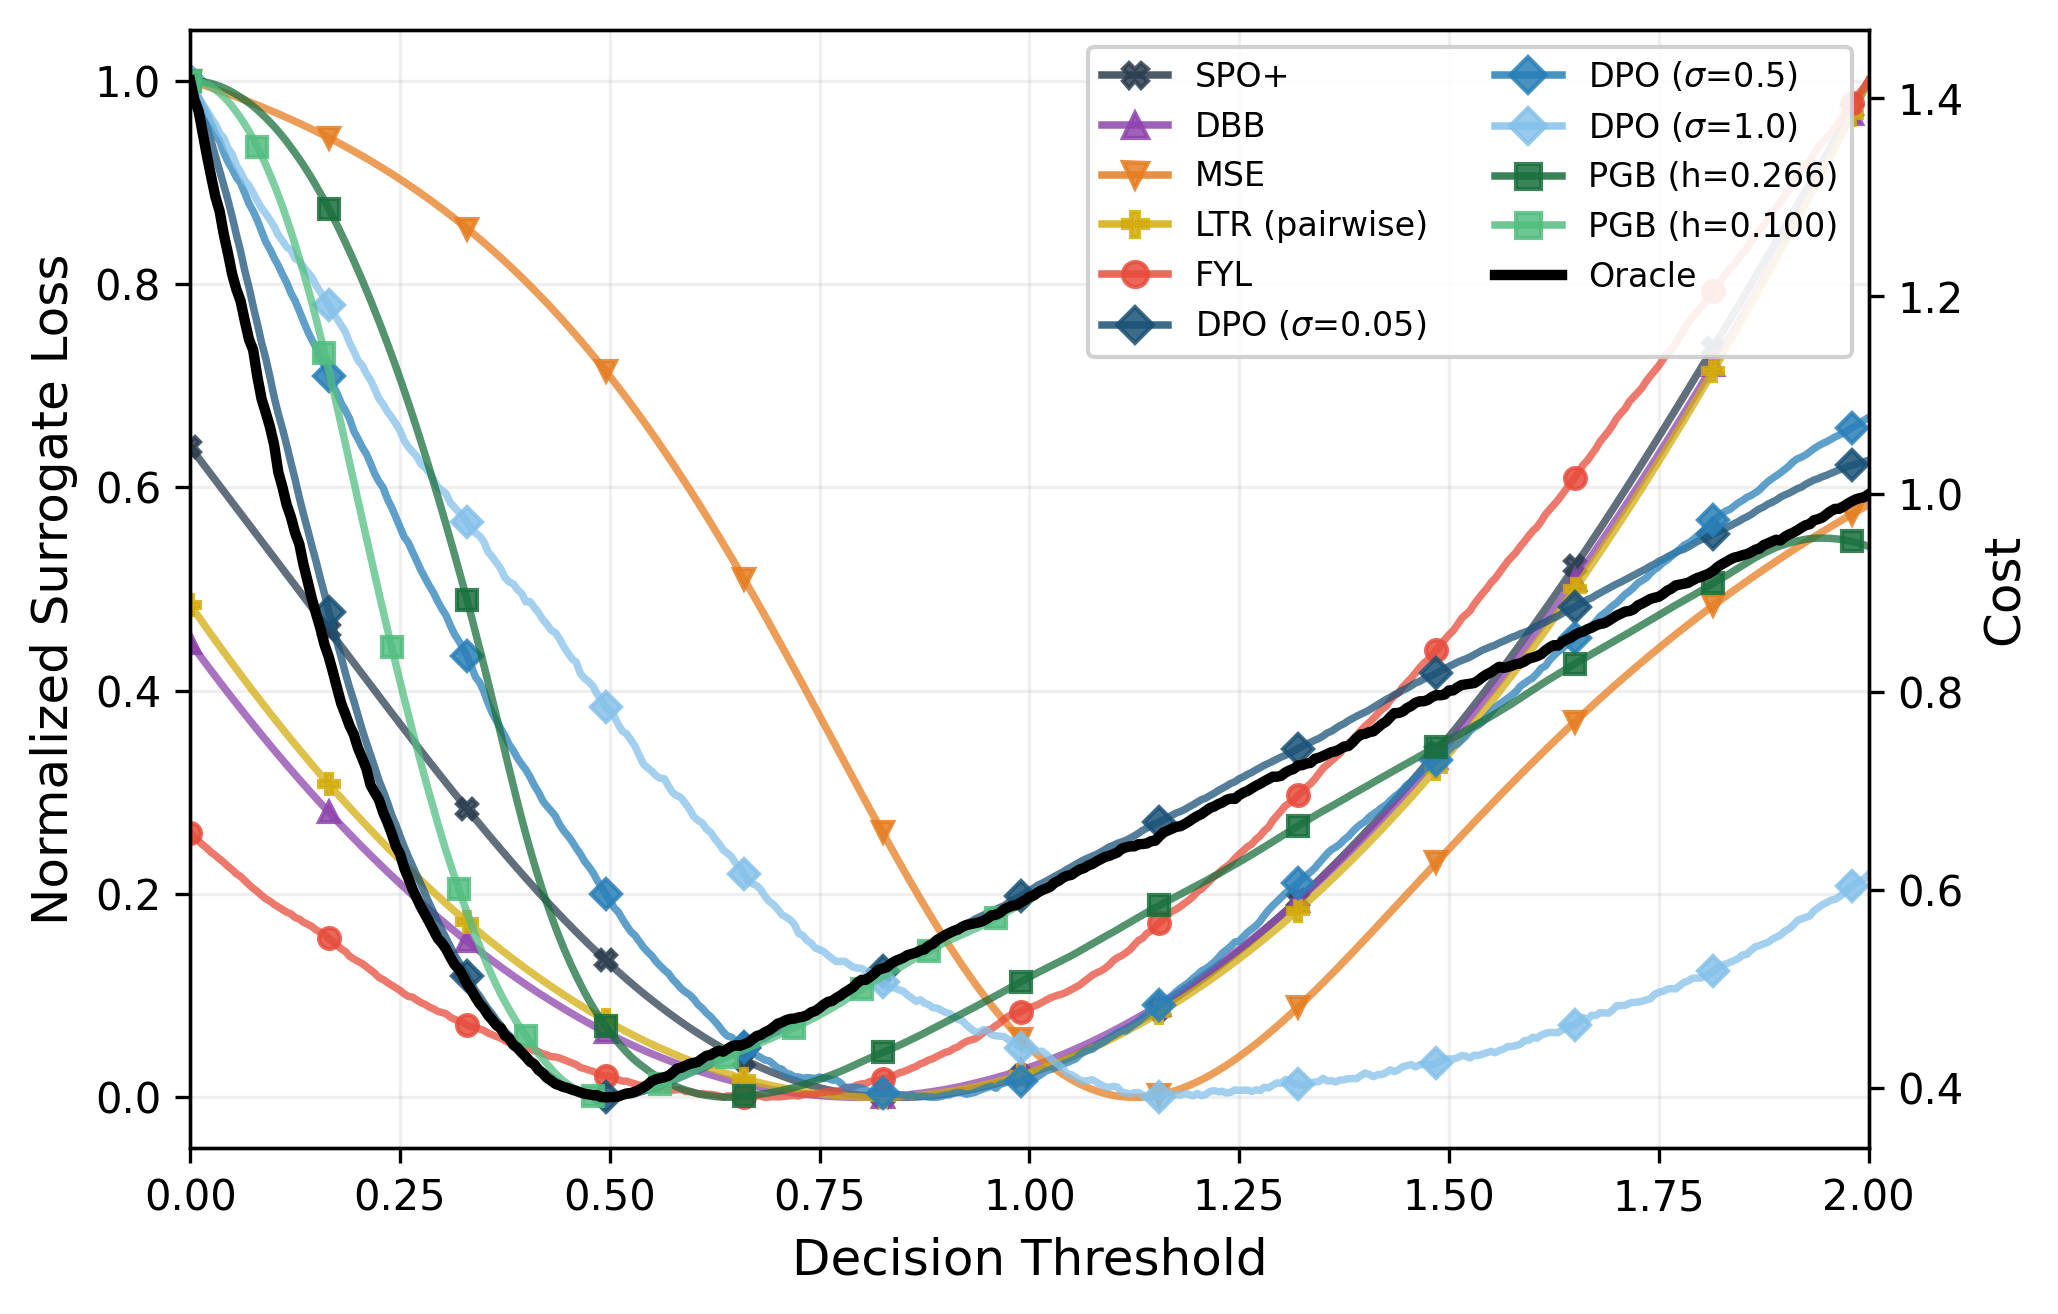
\includegraphics[width=\linewidth]{figures/sweep_v3_noisy.png}
\end{minipage}%
\hfill%
\begin{minipage}[t]{0.27\textwidth}
  \centering
  \vspace{0pt}  
  {\scriptsize
  \renewcommand{\arraystretch}{1.05}
  \resizebox{\linewidth}{!}{%
    \begin{tabular}{lcc}
      \toprule
      Method & Opt.\ thr. & Regret \\
      \midrule
 $\text{PGB}_{h=0.1}$ & 0.50 & 0.39 \\
 $\text{DPO}_{\sigma=0.05}$ & 0.50 & 0.39 \\
 \midrule
  $\text{PGB}_{h=0.266}$ & 0.64 & 0.44 \\
  $\text{DPO}_{\sigma=0.25}$ & 0.68 & 0.45 \\
 FYL & 0.69 & 0.46 \\
 DBB & 0.80 & 0.51 \\
 LTR (pairwise) & 0.82 & 0.52 \\
 SPO{+} & 0.85 & 0.53 \\
 $\text{DPO}_{\sigma=0.5}$ & 0.89 & 0.55 \\
 MSE (2-stage) & 1.0 & 0.59 \\
      \bottomrule
    \end{tabular}%
  }%endresizebox
  }%endscriptsize
\end{minipage}%
\hfill%
\begin{minipage}[t]{0.345\textwidth}
  \centering
  \vspace{0pt}
  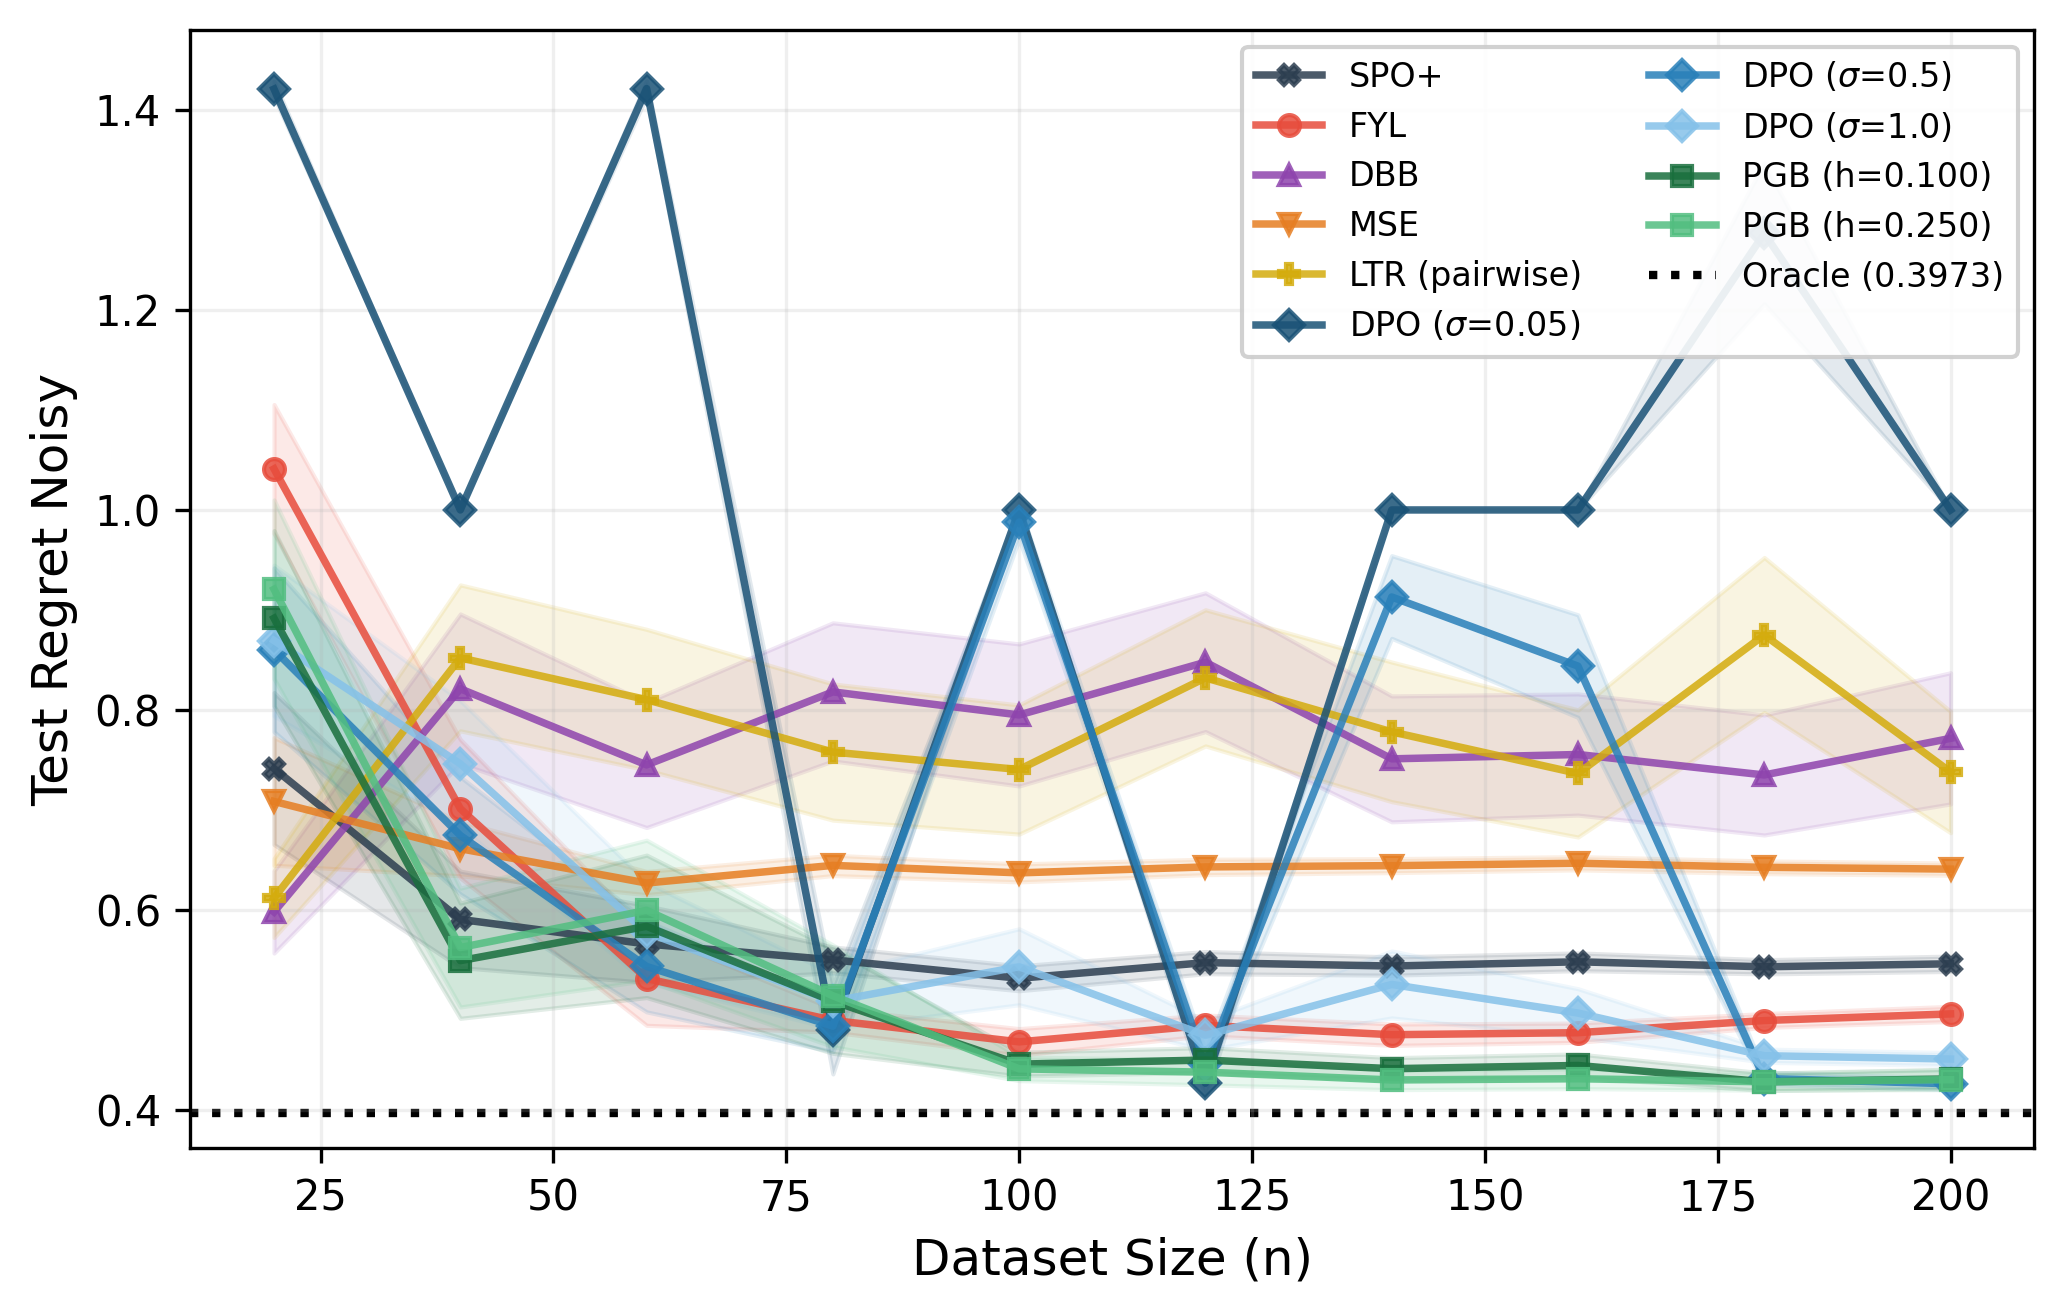
\includegraphics[width=\linewidth]{figures/regret_v3_noisy.png}
\end{minipage}

% Tighten gap between content and caption (local to this figure)
\vspace{-0.25em}
\setlength{\abovecaptionskip}{2pt}
\setlength{\belowcaptionskip}{0pt}

\caption{\textbf{Results on synthetic data under misspecification for various end-to-end PnO methods.} Left: Loss as a function of decision threshold. Ideal methods should match the oracle (solid black), esp. in minima location.
Center: Regret for each method at its optimal $\theta$. 
Right: Regret vs.\ sample size $n$, showing effectiveness of gradient descent for $\theta$.
}%end caption
\label{fig:noisy_synth_triptych}
\end{figure*}